\documentclass[a4paper]{article}
\usepackage[spanish]{babel}
\usepackage[utf8]{inputenc}
\usepackage{charter}   % tipografia
\usepackage{graphicx}
\usepackage{amsmath}
\usepackage{bm}

%%%%%%%LO AGREGUE%%%%%%%%%%  Y yo lo modifique
%\usepackage{hyperref}
%%%%%%%%%%%%%%%%%%%%%%%%%%

\usepackage[bookmarks = true, colorlinks=true, linkcolor = black, citecolor = black, menucolor = black, urlcolor = blue]{hyperref} 




%\usepackage{makeidx}
\usepackage{paralist} %itemize inline
\usepackage[ruled,vlined]{algorithm2e}
%\usepackage{float}
%\usepackage{amsmath, amsthm, amssymb}
%\usepackage{amsfonts}
%\usepackage{sectsty}
%\usepackage{charter}
%\usepackage{wrapfig}
%\usepackage{listings}
%\lstset{language=C}


\usepackage{color} % para snipets de codigo coloreados
\usepackage{fancybox}  % para el sbox de los snipets de codigo

\definecolor{litegrey}{gray}{0.94}

% \newenvironment{sidebar}{%
% 	\begin{Sbox}\begin{minipage}{.85\textwidth}}%
% 	{\end{minipage}\end{Sbox}%
% 		\begin{center}\setlength{\fboxsep}{6pt}%
% 		\shadowbox{\TheSbox}\end{center}}
% \newenvironment{warning}{%
% 	\begin{Sbox}\begin{minipage}{.85\textwidth}\sffamily\lite\small\RaggedRight}%
% 	{\end{minipage}\end{Sbox}%
% 		\begin{center}\setlength{\fboxsep}{6pt}%
% 		\colorbox{litegrey}{\TheSbox}\end{center}}

\newenvironment{codesnippet}{%
	\begin{Sbox}\begin{minipage}{\textwidth}\sffamily\small}%
	{\end{minipage}\end{Sbox}%
		\begin{center}%
		\vspace{-0.4cm}\colorbox{litegrey}{\TheSbox}\end{center}\vspace{0.3cm}}



\usepackage{fancyhdr}
\pagestyle{fancy}

%\renewcommand{\chaptermark}[1]{\markboth{#1}{}}
\renewcommand{\sectionmark}[1]{\markright{\thesection\ - #1}}

\fancyhf{}

\fancyhead[LO]{Sección \rightmark} % \thesection\ 
\fancyfoot[LO]{\small{Agustina Aldasoro, Francisco Noriega, Ezequiel Zimenspitz, Brian Zuker}}
\fancyfoot[RO]{\thepage}
\renewcommand{\headrulewidth}{0.5pt}
\renewcommand{\footrulewidth}{0.5pt}
\setlength{\hoffset}{-0.8in}
\setlength{\textwidth}{16cm}
%\setlength{\hoffset}{-1.1cm}
%\setlength{\textwidth}{16cm}
\setlength{\headsep}{0.5cm}
\setlength{\textheight}{25cm}
\setlength{\voffset}{-0.7in}
\setlength{\headwidth}{\textwidth}
\setlength{\headheight}{13.1pt}

\renewcommand{\baselinestretch}{1.1}  % line spacing


% \setcounter{secnumdepth}{2}
\usepackage{underscore}
\usepackage{caratula}
%\usepackage{url}
\usepackage{hyperref}

% ******************************************************** %
%              TEMPLATE DE INFORME ORGA2 v0.1              %
% ******************************************************** %
% ******************************************************** %
%                                                          %
% ALGUNOS PAQUETES REQUERIDOS (EN UBUNTU):                 %
% ========================================
%                                                          %
% texlive-latex-base                                       %
% texlive-latex-recommended                                %
% texlive-fonts-recommended                                %
% texlive-latex-extra?                                     %
% texlive-lang-spanish (en ubuntu 13.10)                   %
% texlive-science										  %
% ******************************************************** %



\begin{document}


\thispagestyle{empty}
\materia{Algoritmos y Estructuras de Datos III}
\submateria{Primer Cuatrimestre de 2015}
\titulo{Trabajo Práctico II}
%\subtitulo{subtitulo del trabajo}
\integrante{Aldasoro Agustina}{86/13}{agusaldasoro@gmail.com}
\integrante{Noriega Francisco}{660/12}{frannoriega.92@gmail.com}
\integrante{Zimenspitz Ezequiel}{155/13}{ezeqzim@gmail.com}
\integrante{Zuker Brian}{441/13}{brianzuker@gmail.com}


\maketitle
\newpage

\thispagestyle{empty}
\vfill
\begin{abstract}


Habi\'endonos sido dado una serie de tres problem\'aticas a resolver, se plantean sus respectivas soluciones acorde a los requisitos pedidos. Se adjunta una descripci\'on de cada problema y su soluci\'on, conjunto a su an\'alisis de correctitud y de complejidad sumado a su experimentaci\'on. El lenguaje elegido para llevar a cabo el trabajo es C++.

Dentro de cada \emph{.cpp} est\'a el comando para compilar cada ejercicio desde la carpeta donde se encuentran los mismos. A continuaci\'on se los adjunta. El flag \emph{-std=c++11} debi\'o ser a\~nadido  dado que utilizamos la librer\'ia $<$chrono$>$, la cual nos permiti\'o medir tiempos de ejecuci\'on:
\begin{enumerate}
\item \emph{g++ -o main Dakkar.cpp -std=c++11}

\item \emph{g++ -o main Zombieland.cpp -std=c++11}

\item \emph{g++ -o main RefinandoPetroleo.cpp -std=c++11}
	
\end{enumerate}


\end{abstract}

\thispagestyle{empty}
\vspace{3cm}
\tableofcontents
\newpage


%\normalsize
\newpage
\section{Dakkar}
\subsection{Descripci\'on de la problem\'atica}
\subsection{Resoluci\'on propuesta y justificaci\'on}
\subsection{An\'alisis de la complejidad}
\subsection{C\'odigo fuente}
\subsection{Experimentaci\'on}

\subsubsection{Constrastaci\'on Emp\'irica de la complejidad}
\newpage
\section{Zombieland II}
\subsection{Descripci\'on de la problem\'atica}
\subsection{Resoluci\'on propuesta y justificaci\'on}
\subsection{An\'alisis de la complejidad}

\newpage

\subsection{C\'odigo fuente}
	\begin{codesnippet}
	\begin{verbatim}
    struct posYsold {
        int soldadosVivos;
        int i;
        int j;
    };
	\end{verbatim}
	\end{codesnippet}

	\begin{codesnippet}
	\begin{verbatim}
    Matriz ciudadInfestada;
    unsigned int n, m;
    
    int main(int argc, char const *argv[]){
        unsigned int s;
        cin >> n >> m >> s;
        unsigned int inicioH, inicioV, bunkerH, bunkerV;
        cin >> inicioH >> inicioV >> bunkerH >> bunkerV;
        inicioV--;
        inicioH--;
        bunkerV--;
        bunkerH--;
    //la matriz de la ciudad guarda cuantos zombies tiene el eje para moverse
    // a la derecha y hacia abajo (en ese orden)
    //para la izquierda es ir al de la izquierda y preguntar por el derecho
    //para arriba es ir al de arriba y preguntar por el de abajo
        ciudadInfestada = Matriz(n, vector<pair<int, int> >(m));
        for (int i = 0; i < n-1; ++i) {
            for (int j = 0; j < m-1; ++j) {
                cin >> ciudadInfestada[i][j].first;
            }
    //no hay camino a la derecha
            ciudadInfestada[i][m-1].first = -1;
            for (int j = 0; j < m; ++j) {
                cin >> ciudadInfestada[i][j].second;
            }
        }
        for (int j = 0; j < m-1; ++j) {
            cin >> ciudadInfestada[n-1][j].first;
    //no hay camino hacia abajo
            ciudadInfestada[n-1][j].second = -1;
        }
    //no hay camino a la derecha ni abajo
        ciudadInfestada[n-1][m-1].first = -1;
        ciudadInfestada[n-1][m-1].second = -1;
    //creamos el cubo a completar
        Cubo grafo(n, vector<vector<pair<posYsold, bool> > >(m));
        for (int i = 0; i < n; ++i) {
            for (int j = 0; j < m; ++j) {
                grafo[i][j] = vector<pair<posYsold, bool> >(s+1);
            }
        }
    //aplicamos el algoritmo
        int soldadosVivos = zombieland(grafo, inicioH, inicioV, bunkerH, bunkerV, s);
	\end{verbatim}
	\end{codesnippet}

	\begin{codesnippet}
	\begin{verbatim}
    //cout pedido
        cout << soldadosVivos << endl;
        deque<posYsold> recorrido;
    //para armarlo desde el principio hasta el final
        if(soldadosVivos != 0){
            posYsold posActual;
            posActual.soldadosVivos = soldadosVivos;
            posActual.i = bunkerH;
            posActual.j = bunkerV;
            while(posActual.i != inicioH || posActual.j != inicioV){
                recorrido.push_front(posActual);
                posActual = grafo[posActual.i][posActual.j][posActual.soldadosVivos].first;
            }
            posActual.soldadosVivos = s;
            posActual.i = inicioH;
            posActual.j = inicioV;
            recorrido.push_front(posActual);
        }
        for (int i = 0; i < recorrido.size(); ++i) {
            cout << recorrido[i].i+1 << " " << recorrido[i].j+1 << endl;
        }
        return 0;
    }
	\end{verbatim}
	\end{codesnippet}

	\begin{codesnippet}
	\begin{verbatim}
    int zombieland(Cubo& grafo, int inicioH, int inicioV, int bunkerH, int bunkerV, int soldados){
        int maxSoldados = 0;
    //cola para el BFS arranca con la posicion de donde salimos
        queue<posYsold> cola;
        posYsold actual;
        actual.soldadosVivos = soldados;
        actual.i = inicioH;
        actual.j = inicioV;
        cola.push(actual);
    //se marca esta posicion como visitada
        grafo[inicioH][inicioV][soldados].second = true;
        int zombies;
        int resultadoBatalla;
    //mientras tengamos algo para visitar (no sabemos si llegaremos al final)
        while(cola.size() > 0){
    //actual es el primero de la cola
            actual = cola.front();
        //si no estamos el final vemos si podemos ir a cada una de las cuatro direcciones
        //si es valido, no se mueren todos los soldados y no visite ese nodo, 
        //agregare el siguiente nodo a visitar
        //si ya lo visite, existe un camino que me lleva hasta ahi, 
        //ya fue encolado el camino que le sigue
            if(!(actual.i == bunkerH && actual.j == bunkerV)){
                zombies = zombiesCuadra(actual.i, actual.j, ARRIBA);
                resultadoBatalla = resulBatalla(actual.soldadosVivos, zombies);
                if(zombies != -1 && resultadoBatalla > 0 && !grafo[actual.i-1][actual.j]
                [resultadoBatalla].second){
                    posYsold arriba;
                    arriba.soldadosVivos = resultadoBatalla;
                    arriba.i = actual.i-1;
                    arriba.j = actual.j;
                    cola.push(arriba);
                    grafo[actual.i-1][actual.j][resultadoBatalla].second = true;
                    grafo[actual.i-1][actual.j][resultadoBatalla].first = actual;
                }
                zombies = zombiesCuadra(actual.i, actual.j, DER);
                resultadoBatalla = resulBatalla(actual.soldadosVivos, zombies);
                if(zombies != -1 && resultadoBatalla > 0 && !grafo[actual.i][actual.j+1]
                [resultadoBatalla].second){
                    posYsold der;
                    der.soldadosVivos = resultadoBatalla;
                    der.i = actual.i;
                    der.j = actual.j+1;
                    cola.push(der);
                    grafo[actual.i][actual.j+1][resultadoBatalla].second = true;
                    grafo[actual.i][actual.j+1][resultadoBatalla].first = actual;
                }
	\end{verbatim}
	\end{codesnippet}

	\begin{codesnippet}
	\begin{verbatim}
                zombies = zombiesCuadra(actual.i, actual.j, ABAJO);
                resultadoBatalla = resulBatalla(actual.soldadosVivos, zombies);
                if(zombies != -1 && resultadoBatalla > 0 && !grafo[actual.i+1][actual.j]
                [resultadoBatalla].second){
                    posYsold abajo;
                    abajo.soldadosVivos = resultadoBatalla;
                    abajo.i = actual.i+1;
                    abajo.j = actual.j;
                    cola.push(abajo);
                    grafo[actual.i+1][actual.j][resultadoBatalla].second = true;
                    grafo[actual.i+1][actual.j][resultadoBatalla].first = actual;
                }
                zombies = zombiesCuadra(actual.i, actual.j, IZQ);
                resultadoBatalla = resulBatalla(actual.soldadosVivos, zombies);
                if(zombies != -1 && resultadoBatalla > 0 && !grafo[actual.i][actual.j-1]
                [resultadoBatalla].second){
                    posYsold izq;
                    izq.soldadosVivos = resultadoBatalla;
                    izq.i = actual.i;
                    izq.j = actual.j-1;
                    cola.push(izq);
                    grafo[actual.i][actual.j-1][resultadoBatalla].second = true;
                    grafo[actual.i][actual.j-1][resultadoBatalla].first = actual;
                }
            }
        //si llegamos al final, actualizamos los soldados que quedaron vivos, 
        //si es mayor a haber llegado por otro camino
            else
                if(maxSoldados < actual.soldadosVivos)
                    maxSoldados = actual.soldadosVivos;
        //desencolo el nodo que estaba analizando
            cola.pop();
        }
        return maxSoldados;
    }
	\end{verbatim}
	\end{codesnippet}

	\begin{codesnippet}
	\begin{verbatim}
    int zombiesCuadra(int i, int j, movimiento mov){
    //devuelve los zombies que en la cuadra pedida
        switch(mov){
            case ARRIBA:
                if(i == 0)
                    return -1;
                return ciudadInfestada[i-1][j].second;
            case ABAJO:
                return ciudadInfestada[i][j].second;
            case IZQ:
                if(j == 0)
                    return -1;
                return ciudadInfestada[i][j-1].first;
            case DER:
                return ciudadInfestada[i][j].first;
        }
    }
	\end{verbatim}
	\end{codesnippet}

	\begin{codesnippet}
	\begin{verbatim}
    int resulBatalla(int sold, int zomb){
    //devuelve si es posible pasar por una cuadra
        if(sold>=zomb)
            return sold;
        return sold-(zomb-sold); 
    }
	\end{verbatim}
	\end{codesnippet}

\newpage

\subsection{Experimentaci\'on}
\subsubsection{Constrastaci\'on Emp\'irica de la complejidad}
Para realizar los experimentos, se consideró como peor caso, aquel en el que se debiera recorrer cada nodo de la ciudad, tantas veces como cantidad de soldados se tuviese a disposicion, siendo ese caso, en el que se recorrerían $s.n.m$ elementos, coiniciendo así con la complejidad teórica $O(s.n.m)$.\\
Aunque ese el caso deseable, generar dicha instancia para los distintos valores de $s$, $n$ y $m$, resultó tan dificultoso como resolver el problema en cuestión.\\
Por ello, se decidio generar instancias con una cantidad aleatoria de zombies por cuadra. Ésto permitió generar instancias automáticamente, para casos de prueba grandes, pero trajo consigo los siguientes problemas:
\begin{enumerate}
	\item No se puede determinar si existe un camino desde el punto de inicio hasta el búnker.
	\item No se puede determinar, si al existir un camino, este será único.
	\item No se puede determinar cuantos soldados van a llegar al búnker.
	\item No se puede determinar cuantos caminos adulteran la cantidad de soldados, ni cuantos soldados mueren en cada uno de ellos.
\end{enumerate}

El resultado del generador de instancias, proporcionaba un laberinto como el siguiente:

\begin{center}

\includegraphics[width=7cm,keepaspectratio=yes]{imagenes/ej2/maze.png}
\end{center}

Los pasajes del laberinto son los caminos donde hay entre $0$ y $s+1$ zombies, y las paredes, caminos donde hay entre $0$ y $s$.2.\\
Estos valores aleatorios fueron tomados adrede, por un lado, para que incluso el mejor camino (alguno de los pasajes que conducen a la salida), tuviera perdida de soldados, pero intentando que éstas sean mínimas, para aumentar las probabilidades de que puedan efectivamente llegar al búnker.
Las paredes, no son un obstaculo, dado que podrían terminar siendo un pasaje, pero la probabilidad de que eso ocurra es muy baja.\\
Aún asi, el $s$ tomado en el algoritmo aleatorio es el que se recibe en la entrada. Esto significa, que se configura al principio, y despues no se actualiza con la cantidad de soldados despues de una batalla.\\
Por ende, no podemos determinar el porcentaje de soldados totales que llegarán, pero sí podemos saber el porcentaje que sobrevivirá a la primer batalla.\\
Así, la cantidad de soldados que sobreviviran a la primer batalla es:
\begin{itemize}
	\item 95\% en caso de que el camino sea un pasaje.
	\item 50\% en casos de que el camino sea una pared.
\end{itemize}
Estos rangos aleatorios también se obtuvieron experimentando, hasta lograr valores que ocasionaran bajas pero que no impidieran a los soldados llegar al búnker en la mayoría de los casos. Dichos experimentos exceden el interés de esta sección y no serán discutidos.\\

Pese a dificultades expuestas, se decidió proceder con dichas instancias, ya que lograban generar una fluctuación en la cantidad de soldados, y esto, si bien lejos del peor caso propuesto, resultó ser una aproximación que nos resultó suficiente.\\

Por lo dicho anteriormente, se realizaron experimentos sobre los siguientes dos casos:
\begin{itemize}
	\item \textbf{Cero zombies}: En esta instancia, la cantidad de zombies en cada cuadra es cero, con lo cual, el algoritmo recorre toda la ciudad, y se queda con cualquier camino.
	\item \textbf{Zombies aleatorios}: Es la instancia explicada anteriormente.
\end{itemize}

También es necesario aclarar, que los experimentos se realizaron sobre ciudades cuadradas, con puntos de inicio y llegada en los extremos opuestos de la ciudad, y con cantidad de soldados iniciales igual a 20.\\

A continuación se detallan los experimentos y sus resultados.
Debido al tamaño de las instancias de prueba, los inputs de dichos experimentos no fueron adjuntados.
\begin{center}
	\begin{tabular}{|c|c|c|}
	\hline
	Experimento & \textbf{Cero zombies} & \textbf{Zombies aleatorios}\\
	\hline
	\hline
	Tamaño de la ciudad & \multicolumn{2}{|c|}{Soldados al final}\\
	\hline
	50x50 & 20 & 6\\
	\hline
	100x100 & 20 & 19\\
	\hline
	250x250 & 20 & 17\\
	\hline
	500x500 & 20 & 17\\
	\hline
	750x750 & 20 & 16\\
	\hline
	1000x1000 & 20 & 12\\
	\hline
	1250x1250 & 20 & 20\\
	\hline
	1500x1500 & 20 & 7\\
	\hline
	1750x1750 & 20 & 14\\
	\hline
	2000x2000 & 20 & 20\\
	\hline
	\end{tabular}
\end{center}

Dado que los tiempos de ejecución para ambos experimentos varían ampliamente, primero analizaremos el experimento de \textbf{Cero zombies}.

\includegraphics[width=15cm,keepaspectratio=yes]{imagenes/ej2/czneto.png}

Como se puede apreciar, al no haber zombies, no existe ningun camino en el cual mueran soldados, por lo que los tiempos se incrementan acorde a la dimension de la ciudad, y al ser cuadradas, crece polinomialmente.

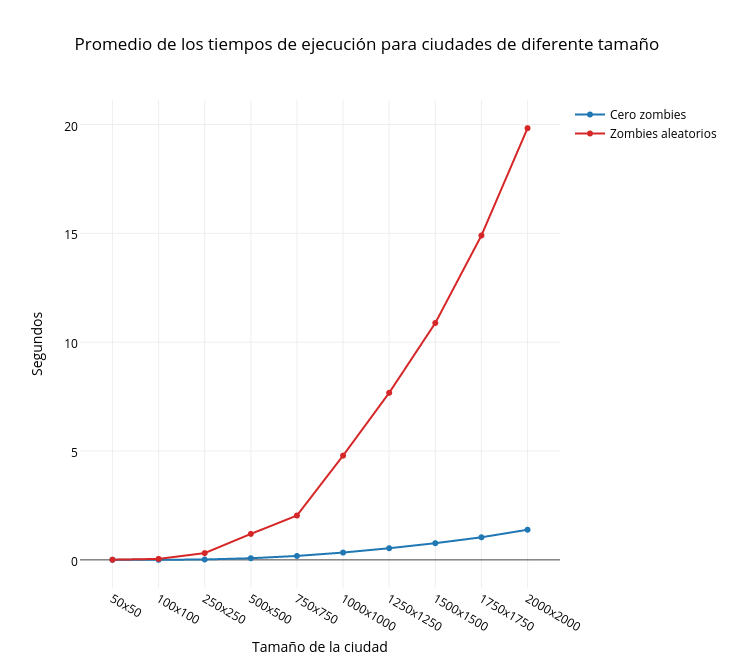
\includegraphics[width=15cm,keepaspectratio=yes]{imagenes/ej2/czyza.png}

Aquí se pueden apreciar las diferencias de tiempos. Ésta radica en el hecho de que \textbf{Zombies aleatorios} posee caminos en los cuales los soldados mueren. Por ello, el algoritmo deberá recorrer, en peor caso, $s$ veces la ciudad entera.\\

Se procedió, entonces, a dividir los resultados de \textbf{Zombies aleatorios} por la cantidad de soldados iniciales con los que se ejecutó el algoritmo a fin de que quede reflejado, que en ese caso, los tiempos serán muy similares a los de \textbf{Cero zombies}. Esto se debe a que ya no son los tiempos de recorrer $s$ veces la ciudad, sino de recorrerla una sola vez.
Sin embargo, es necesario aclarar que la similitud que se intenta mostrar, es aproximada, ya que no podemos asegurar que efectivamente, el algoritmo recorre $s$ veces la ciudad. Tal es el peor caso, y como hemos expuesto en un principio, no podemos asegurar que sea el que realmente ocurre.

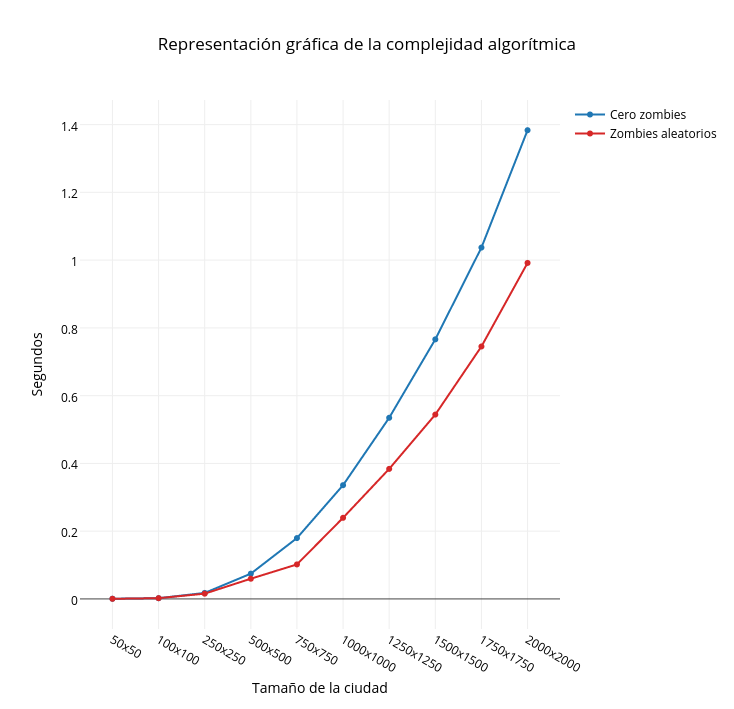
\includegraphics[width=15cm,keepaspectratio=yes]{imagenes/ej2/zaczados.png}

Manteniendo los resultados de \textbf{Zombies aleatorios} divididos por $s$, finalmente dividimos los resultados tanto de \textbf{Cero zombies} como de \textbf{Zombies aleatorios}, por $n$, y en una instancia aparte, por $n.m$.
De esta manera, dado que en ambos tienen $s$ igual a 1, solo queda ver que al dividir por $n$, los resultados se aproximan a una función lineal, y que al dividirlos por $n.m$, se aproximan a una constante.\\

Como solo nos interesa la relación, y no la función exacta ni la constante, multiplicamos los resultados de dichas divisiones por 100, para que los valores sean más claros y visibles.

\includegraphics[width=15cm,keepaspectratio=yes]{imagenes/ej2/linealizacion.png}

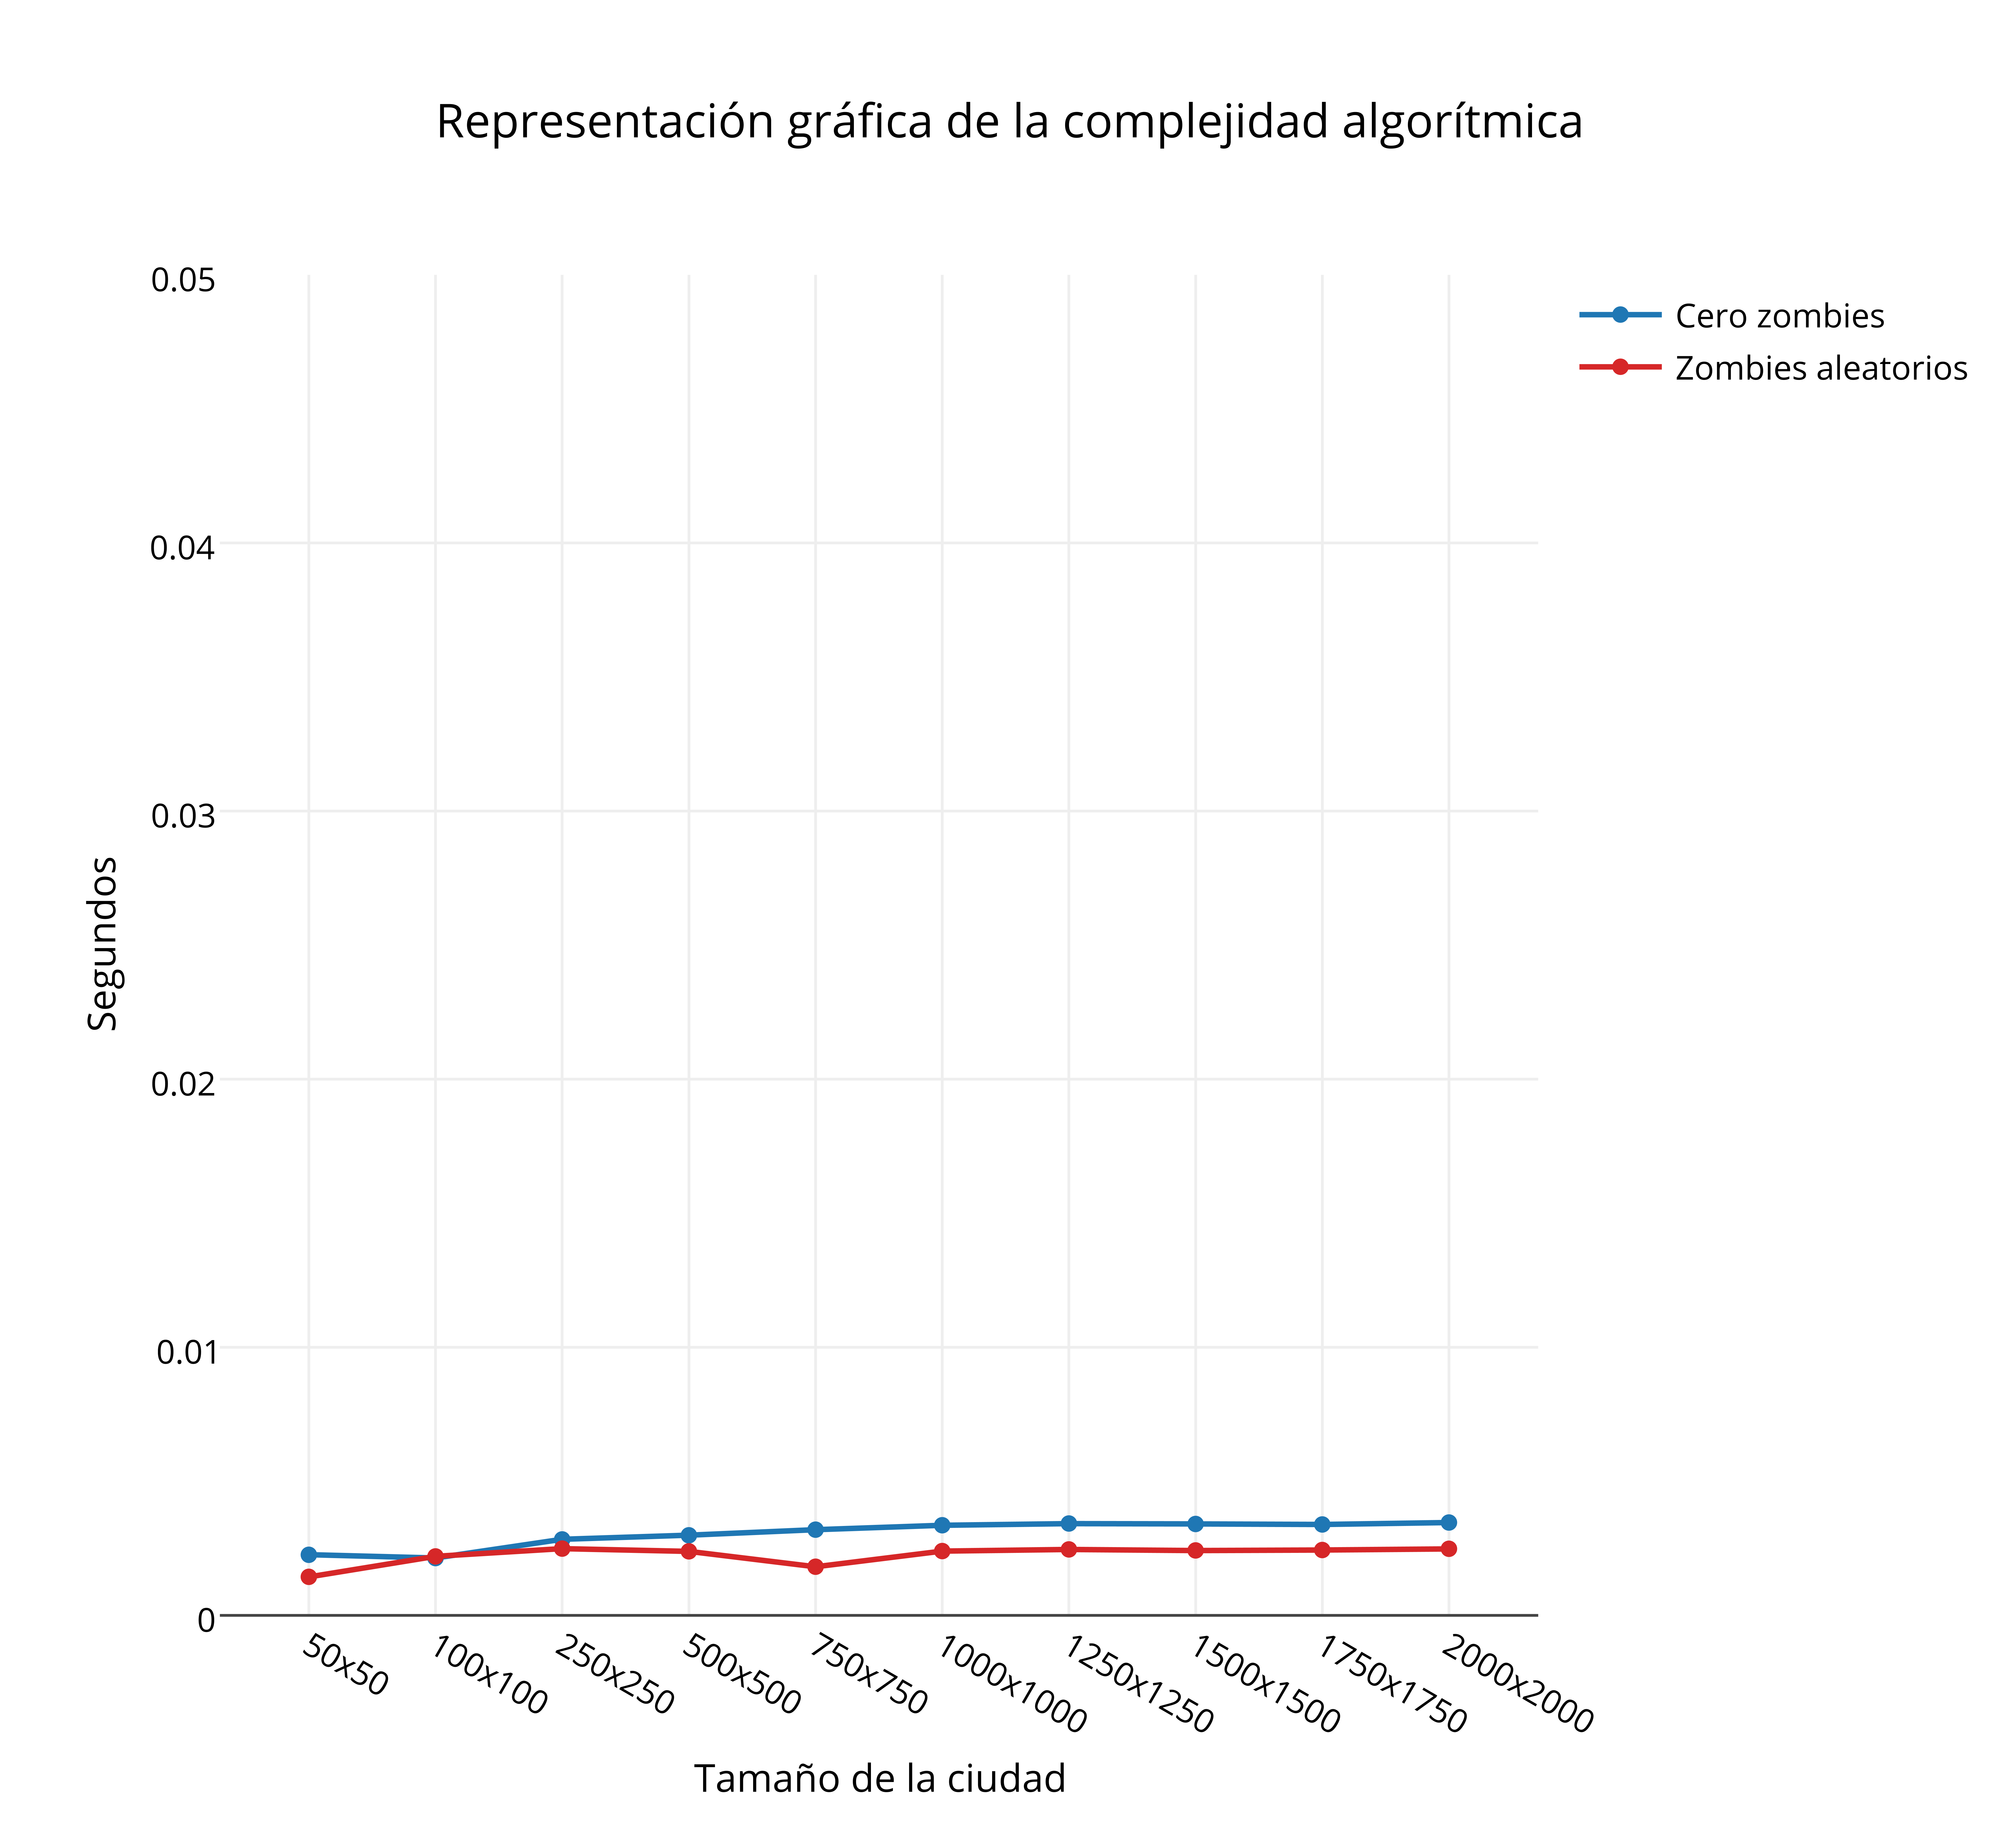
\includegraphics[width=15cm,keepaspectratio=yes]{imagenes/ej2/constantizacion.png}

Se puede ver que la experimentación se corresponde con la teoría, y que la complejidad, en peor caso, es $O(s.n.m)$.


\newpage
\section{Heur\'istica Constructiva Golosa} \label{ej3}
\subsection{Explicaci\'on}
La heurística constructiva golosa busca, dado un grafo, determinar un conjunto independiente dominante mínimo. 

Para ello, el algoritmo ordena los nodos de acuerdo al grado de cada uno de ellos, de mayor a menor. Este orden se establece al comienzo de la ejecución y no se actualiza.\\

Luego, recorre dichos nodos, y por cada uno de ellos, lo agrega al conjunto solución, y va eliminando a sus vecinos, hasta que no quedan más nodos.\\

De esta manera, el algoritmo siempre obtiene un conjunto independiente (dado que por cada nodo que toma, elimina a sus vecinos) y dominante (dado que por cada nodo que toma, lo agrega al conjunto, y elimina a sus vecinos, es decir, que estos son adyacentes a un nodo del conjunto), pero no puede asegurar que siempre sea mínimo. Eso dependerá del grafo.\\

\textcolor{red}{Falta una explicacion mas detallada (un pseudocodigo, o algo), y aclarar que es goloso porque en cada paso elige la mejor opcion y nosostros definimos MEJOR como el mayor grado total}
%Explicar detalladamente el algoritmo implementado.

\newpage
\subsection{Complejidad Temporal}\label{compej3}
\textcolor{red}{Aca no me meto, todavia...}

En lo que respecta a la complejidad temporal, demostraremos a continuación que la misma es $O(n^{2})$ en la cantidad de nodos del grafo.\\

Recordemos que el algoritmo ordena los nodos de mayor grado a menor grado, luego toma el primero de dicha lista, lo agrega al conjunto solución, y lo elimina de la lista junto a sus adyacentes. Luego repite el proceso, tomando el siguiente nodo de la lista de nodos restantes.\\
Dicho esto, definiremos a $f(i,n): \mathbb{N} \rightarrow \mathbb{N}$ como:

$f(i,n)$ = Cantidad de operaciones en el peor caso, teniendo $n$ nodos totales y faltando eliminar $i$.\\
Es decir,\par
\begin{itemize}
	\item$f(0,n) = c$, dado que no falta eliminar ningun nodo, el algoritmo termina, con $c$ alguna cantidad constante de operaciones.\par
	\item $(\forall i \in {1...n-1}) f(i,n) = h*(i-1) + f(i-1,n) + c$, con $h$ la cantidad de vecinos del nodo que estoy viendo, $c$ alguna cantidad constante de operaciones, y $f(i-1,n)$ es el llamado recursivo.\\
\end{itemize}
Expliquemos que significa cada monomio:
\begin{itemize}
	\item $h*(i-1)$: En el peor de los casos, recorre por cada nodo de la lista de adyacencia del nodo tomado, a los demas nodos sin marcar (sin incluir el nodo tomado).
	\item $f(i-1,n)$: En el peor de los casos, no hay nodos de la lista de adyacencia, que no hayan sido eliminados aún.
	\item $c$: Alguna cantidad constante de operaciones.
\end{itemize}
Entonces, querremos demostrar que $(\forall i \in {1...n-1}) f(i,n) \leq k*i*n + c$ (con $k$ y $c$ alguna constante), pues al momento de ejecutar el algoritmo, se tienen $n$ nodos, y faltan eliminar $n$ nodos, siendo la complejidad del mismo, $O(f(n,n)) = O(n^{2})$; y dado que la cantidad de nodos por borrar no puede ser mayor que la cantidad total de nodos, es correcto pedir que $0 \leq i < n$.\\

\newpage
{\large\textbf{Teorema}}\\
Dado $f(i,n): \mathbb{N} \rightarrow \mathbb{N}$ definida como\\
$f(i,n)$ = Cantidad de operaciones  en el peor caso, teniendo $n$ nodos totales y faltando eliminar $i$.\\
$f(0,n) = c$\\
$f(i,n) = h*(i-1) + f(i-1,n) + c$\\
Luego, $(\forall i \in {1...n-1}) f(i,n) \leq k*i*n + c$.\\

{\large\textbf{Demostración}}\\
Sea $P(i) = f(i,n) \leq k*i*n + c$, demostraremos por inducción global, que $(\forall i \in {1...n-1}) P(i)$\\
Entonces,\\
\textbf{Casos base:}
\begin{itemize}
    \item[•] $f(0,n) = c$
    \item[•] $f(1,n) = h*(1-1) + c = c \leq k*1*n + c$\\
    Dado que tengo $n$ nodos, y solo falta eliminar uno. $k$ es alguna cantidad constante de operaciones para eliminar el nodo y finalizar el algoritmo.
\end{itemize}
\textbf{Paso inductivo:}\\

$\underbrace{P(1) \wedge P(2) \wedge ... \wedge P(m-1)}_{\text{Hipótesis inductiva}} \Rightarrow \underbrace{P(m)}_{\text{Tesis inductiva}}$\\

Es decir, que por hipótesis inductiva, podemos suponer que vale $f(r,n) \leq k*r*n + c$, con $r \leq m-1$, y queremos ver que $f(m,n) \leq k*m*n + c$.\\
Luego,
\begin{align*}
f(m,n) & = h*(m-1) + f(m-1,n) + c \\
 \stackrel{HI}{\Longrightarrow} f(m,n) & \leq h*(m-1) + n*(m-1) + c \\
 \intertext{Dado que la cantidad de vecinos adyacentes esta acotada por la cantidad de nodos totales, $0 \leq h < n$, luego}
 & \leq n*(m-1)+n*(m-1) + c\\
 & \leq n*m + n*m + c\\
 & = 2*n*m + c\\
 & \leq \underbrace{k*n*m + c}_{\text{Tesis inductiva}} \text{       En particular, con $k = 2$ en este caso}
\end{align*}
\hfill $\blacksquare$

Entonces, $f(i,n) \leq c*i*n + k$, para algún $c$ y $k$ constantes.
Dado que el algoritmo ejecuta, en peor caso, $f(n,n)$ operaciones, su complejidad esta acotada por $f(n,n)$, por lo tanto, tiene complejidad $O(n^{2})$.\\

También es adecuado decir, que el algoritmo tiene complejidad $\Omega(n*log(n))$, dado que debe ordenar los nodos de acuerdo al grado de cada uno, y cualquier algoritmo de ordenamiento basado en el árbol de decisiones no posee mejor complejidad que la mencionada.

%Calcular el orden de complejidad temporal de peor caso del algoritmo.
\subsection{Comparaci\'on de resultados con soluci\'on \'optima}
La heurística constructiva golosa fallará en encontrar la solución óptima para todos los casos.
Particularmente, existen grafos para los cuales la heurística fallará siempre.\\
Algunos de ellos son:
\textcolor{red}{Insertar nodo radial}

En este ejemplo, el greedy tomará como primer nodo, al nodo del centro, y eliminará a todos sus adyacentes. Luego, tomará todas las componentes conexas restantes.
El resultado final será una solución con $(m-2)*m$ versus $m$ de la solución óptima.

\textcolor{red}{Insertar mas ejemplos... Ayuda...}

%Describir instancias de CIDM para las cuales la heuristica no proporciona una solucion optima. Indicar que tan mala puede ser la solucion obtenida respecto de la solucion optima.
\subsection{Experimentaci\'on}
%Realizar una experimentacion que permita observar la performance del algoritmo en terminos de tiempo de ejecucion en funcion de los parametros de la entrada.
Para la experimentación, se realizaron experimentos sobre grafos generados de manera aleatoria, fijando nodos y variando ejes, y viceversa.

A continuación se adjuntan los gráficos con los resultados:

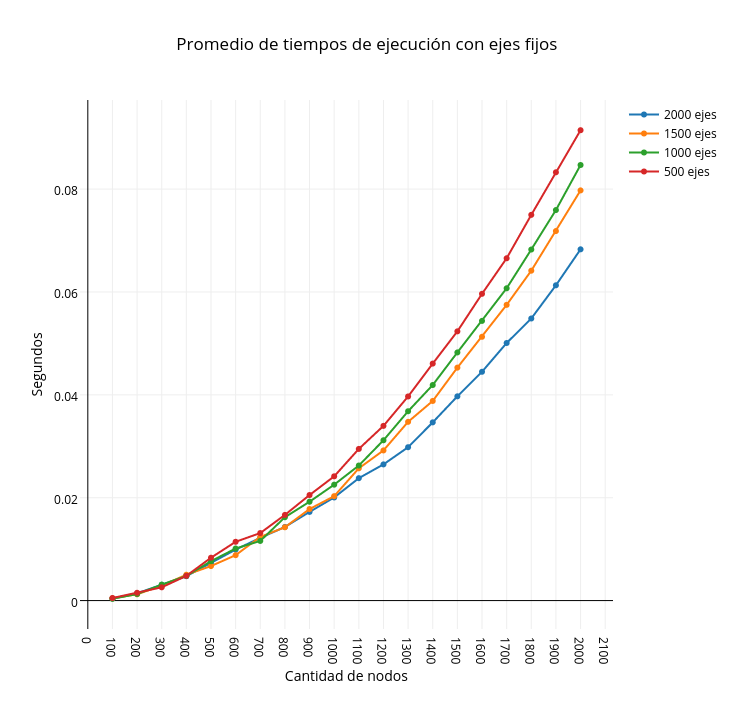
\includegraphics[width=15cm,keepaspectratio=yes]{imagenes/greedy/fixedge.png}

Como se puede observar, los tiempos aumentan a medida que disminuyen la cantidad de ejes. Esto se debe a que a menor cantidad de ejes, menor cantidad de nodos se eliminan de la lista de nodos que itera el algoritmo.

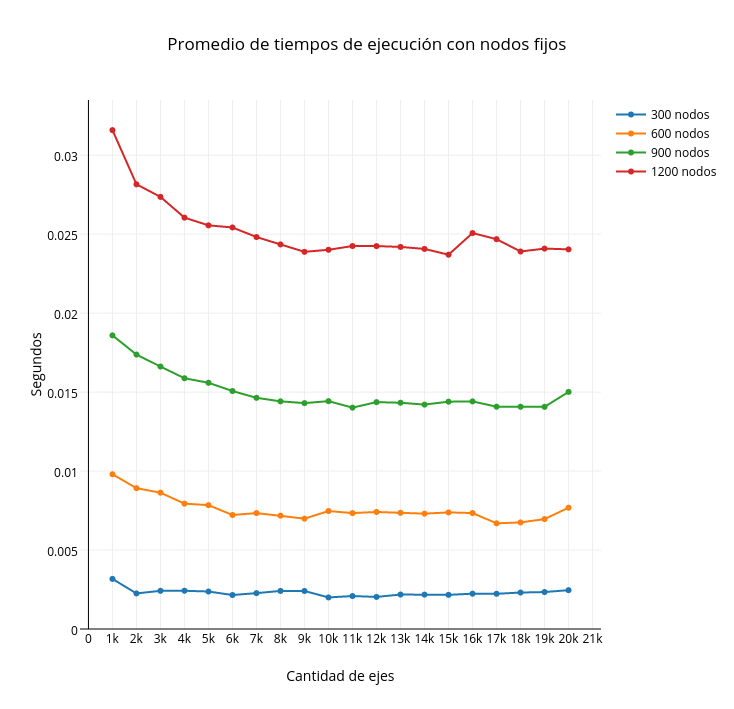
\includegraphics[width=15cm,keepaspectratio=yes]{imagenes/greedy/fixnode.png}

En este gráfico, se puede ver que si bien la cantidad de ejes (como fue mencionado en el gráfico anterior) afecta los tiempos, a mayor cantidad de ejes se puede observar que el verdadero limitante es la cantidad de nodos. Aquí se aprecia que la complejidad teórica se corresponde, en cuanto a que depende de la cantidad de nodos, y no de la cantidad de ejes.

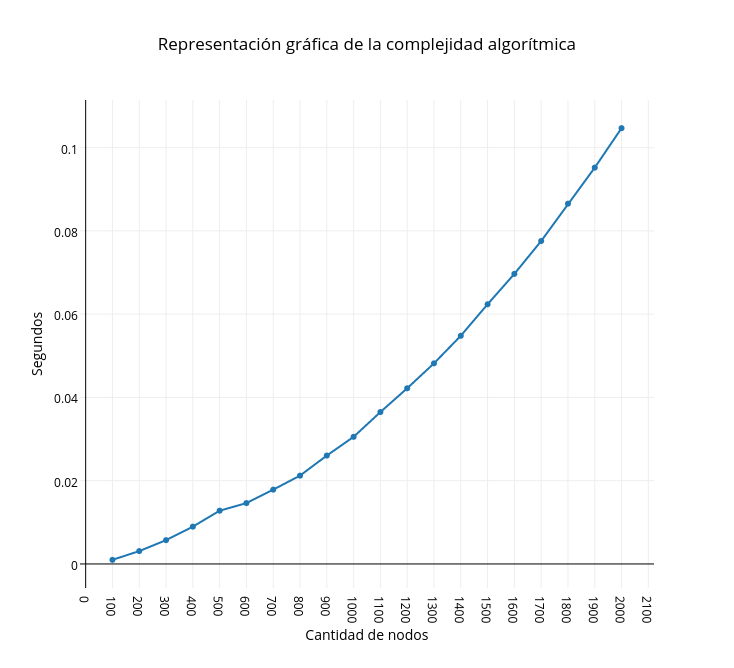
\includegraphics[width=15cm,keepaspectratio=yes]{imagenes/greedy/worst1.png}

Resultó interesante graficar, a su vez, algún caso en el que se refleje la complejidad algorítmica.
Para ello, se tomo el grafo sin ejes, es decir, todas componentes conexas, puesto que el algoritmo deberá recorrer, por cada nodo, el resto de todos los nodos preguntando si son vecinos.
Aquí se puede apreciar que efectivamente, los tiempos incrementan de manera cuadrática.

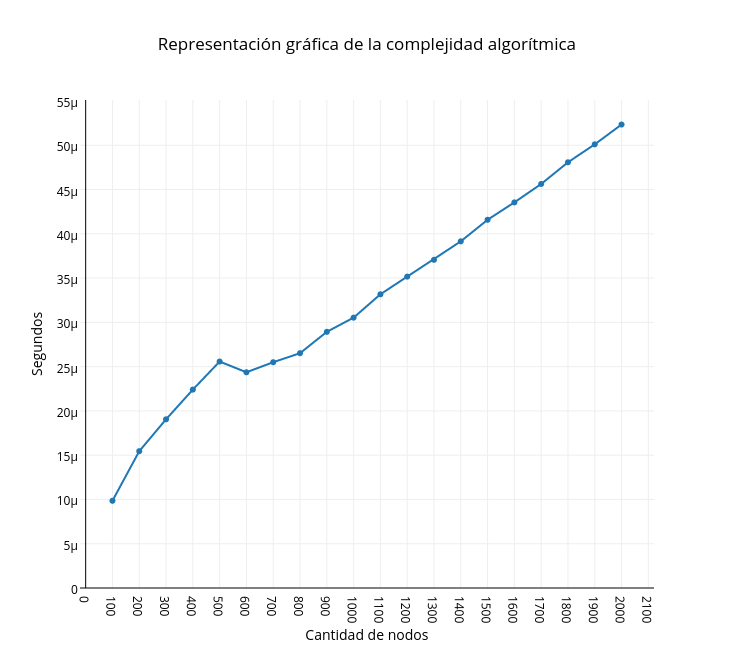
\includegraphics[width=15cm,keepaspectratio=yes]{imagenes/greedy/worst2.png}

Para asegurarnos de que efectivamente la función corresponde a la familia de funciones cuadráticas y no a otra, se procedió a dividir los resultados por el tamaño de la entrada.
Se puede apreciar que el gráfico se aproxima a una función lineal.

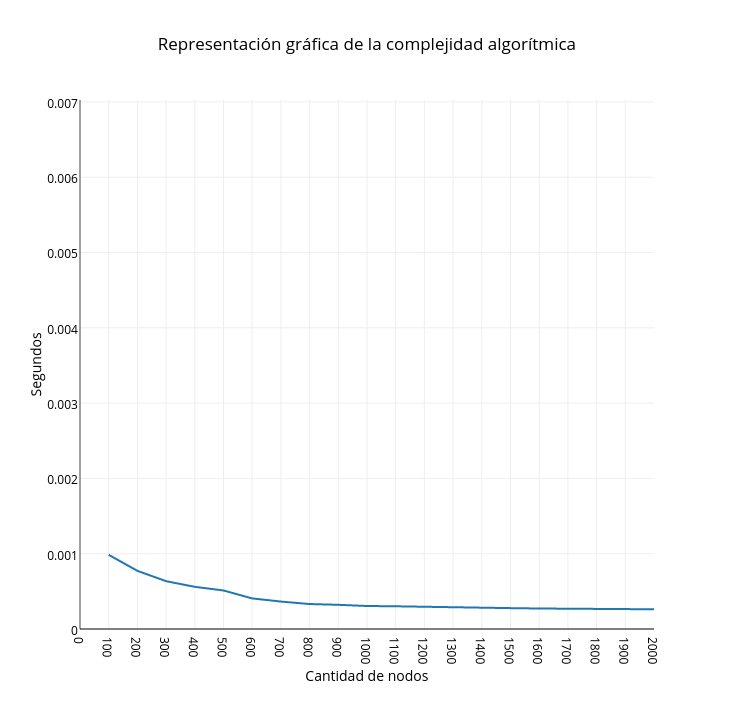
\includegraphics[width=15cm,keepaspectratio=yes]{imagenes/greedy/worst3.png}

Finalmente, se procedió a dividir los resultados (ya divididos) por el tamaño de la entrada nuevamente.
Efectivamente, el resultado tiende a una constante, lo que termina demostrando de manera empírica, la complejidad teórica explicada.
\newpage

% \section{Objetivos generales}

% El objetivo de este Trabajo Práctico es ...


% \section{Contexto}

% \begin{figure}
%   \begin{center}
% 	
\includegraphics[scale=0.66]{imagenes/logouba.jpg}
% 	\caption{Descripcion de la figura}
% 	\label{nombreparareferenciar}
%   \end{center}
% \end{figure}


% \paragraph{\textbf{Titulo del parrafo} } Bla bla bla bla.
% Esto se muestra en la figura~\ref{nombreparareferenciar}.




%Habra que insertar el enunciado???
% %\section{Enunciado y solucion} 
% %\input{enunciado}

% \section{Conclusiones y trabajo futuro}

\end{document}

